%%%%%%%%%%%%%%%%%%%%%%%%%%%%%%%%%%%%%%%%%%%%%%%%%%%%%%%%%%%%%%%%%%%%%%%%
%                                                                      %
%     File: Thesis_Results.tex                                         %
%     Tex Master: Thesis.tex                                           %
%                                                                      %
%     Author: Andre C. Marta                                           %
%     Last modified :  2 Jul 2015                                      %
%                                                                      %
%%%%%%%%%%%%%%%%%%%%%%%%%%%%%%%%%%%%%%%%%%%%%%%%%%%%%%%%%%%%%%%%%%%%%%%%

\chapter{Investing in a new product, allowing a simultaneous production period, when the firm is already active}
\label{chapter:3}


%Insert your chapter material here...

%%%%%%%%%%%%%%%%%%%%%%%%%%%%%%%%%%%%%%%%%%%%%%%%%%%%%%%%%%%%%%%%%%%%%%%%
\section{Introduction}
\label{section:3_intro}

%We increase the complexity of our problem by considering that the firm has three different states of production.

%In the first state, we consider that the firm only produces a (very) \textit{stable} product, that does not depend on the demand observe. We will call it \textit{old} product. Its demand function $p_0$ and instaneous profit function $\pi_0$ are the same as stated in Chapter \ref{chapter:2} and take the values of \eqref{p0} and \eqref{pi0}, respectively.

%In the second state, we consider the firm produces simultaneously the \textit{old} product and a new one. We will call it \textit{new} product. This \textit{new} product is inserted in the market since after the innovation process as achieved a certain innovation level, \textit{a priori} defined. Since it's based on a new technology and it's a product that is not know by people, we will consider that its profit depends on the demand level.

We extend the situation described on the previous chapter by considering a firm, which has an established product in the market, and wants to find the best time to:
\begin{enumerate}
	\item Invest and introduce in the market an innovative product with technology level $\theta$, allowing the possibility of a simultaneous production of both \textit{old} and \textit{new} products;
	\item Abandon the production of the \textit{old} product, maintaining the \textit{new} one in the market.
\end{enumerate}

Consequently, as showed on Figure \ref{3_time}, the firm faces 3 stages.

\vspace{4mm}
\begin{figure}[!htb]
	\centering
	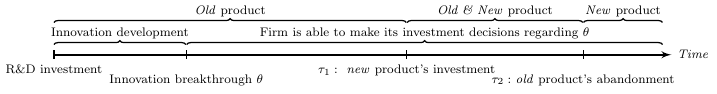
\includegraphics[width=\textwidth]{Prob3/3_timelinet.PNG}
	\caption{Timeline representing the three possible different stages of production and associated decisions.}
	\label{3_time}
\end{figure}
On the first stage only the established\&old product is produced, whose unitary price $p_0$ and profit functions $\pi_0$ are the same as stated in Chapter \ref{chapter:2}, and take the values of \eqref{p0} and \eqref{pi0}, respectively.

During the second stage the firm produces both \textit{old} and \textit{new} products, leading to the follow profit functions
\begin{align}
\pi_0^A(X_t)&=(1-\alpha K_0-\eta K_1 X_t) K_0\\
\pi_1^A(X_t)&=(\theta-\alpha K_1-\eta K_0 X_t) K_1.
\end{align}

A \textit{cannibalisation} (or\textit{ horizontal differentiation}) parameter $\eta$ is introduced on both expressions to embody the crossed effect between the \textit{old} and the \textit{new} product. As we consider both products to be interacting in the same market, $\eta$ represents the penalty that the quantity
associated to a product will influence the price of the other. We consider here
that this influence is the same for both products, so we can have a unique cannibalisation parameter $\eta$.
By observing that $\eta\geq \alpha$ would imply a larger effect on the product price that on the quantity of production itself, we establish $\eta$ to be such that $\eta < \alpha$. 
By adding both profits $\pi^A_0$ and $\pi_1^A$ we attain the profit associated to this second stage, that is,
%Therefore the resultant profit function associated to this second state of production is denoted by $\pi_A$ and it is such that
\begin{equation}
\pi_A(X_t)=\pi_0^A(X_t)+\pi_1^A(X_t)=(1-\alpha K_0)K_0+(\theta-\alpha K_1)K_1X_t-2\eta K_0 K_1 X_t.
\end{equation}
%\begin{align}
%\pi_0^A(X_t)&=(1-\alpha K_0-\eta K_1 X_t) K_0\\
%\pi_1^A(X_t)&=(\theta-\alpha K_1-\eta K_0 X_t) K_1.
%\end{align}

%However this one cannot be greater than the sensibility parameter $\alpha$ ($\eta<\alpha$). Otherwise, the quantity of the other product would have a larger effect on the product price than the quantity of the product itself.




%The instantaneous profit functions associated to the \textit{old} and the \textit{new} product, during the simultaneous production, are given respectively by
%\begin{align}
%\pi_0^A(X_t)&=(1-\alpha K_0-\eta K_1 X_t) K_0\\
%\pi_1^A(X_t)&=(\theta-\alpha K_1-\eta K_0 X_t) K_1.
%\end{align}


%We need to consider a \textit{cannibalisation} (or\textit{ horizontal differentiation}) parameter $\eta$ that corresponds to the crossed effect between the \textit{old} and the \textit{new} product. As we consider both products to be interacting in the same market, $\eta$ represents the penalty that the quantity
%associated to a product will influence the price of the other. We consider here
%that this influence is the same for both products, so we can have a unique cannibalisation parameter $\eta$, however this one cannot be greater than the sensibility parameter $\alpha$ ($\eta<\alpha$). Otherwise, the quantity
%of the other product would have a larger effect on the product price than the quantity of the product itself.

%The instantaneous profit function associated to this second state of production is denoted by $\pi_A$ and it is such that
%\begin{equation}
%\pi_A(X_t)=\pi_0^A(X_t)+\pi_1^A(X_t)= \pi_0+\pi_1(X_t)-2\eta K_0 K_1 X_t=(1-\alpha K_0)K_0+(\theta-\alpha K_1)K_1X_t-2\eta K_0 K_1 X_t.
%\end{equation}


Finally, on the third state, we consider that the firm abandons the \textit{old} product and starts producing solely the \textit{new} product, which is not considered to be a stable product. Its demand function $p_1$ and profit function $\pi_1$ are as stated in Chapter \ref{chapter:2}, and take the values of \eqref{p1} and \eqref{pi1}, respectively.


Therefore we want to find two optimal times to make different (but maybe simultaneous) decisions. We want to find the best time $\tau_1$ to go from the first to the second stage - that is, to invest in the \textit{new} product and start producing, simultaneously, the \textit{old} and the \textit{new} product - and we also want to find the best time $\tau_2$ to go from the second to the third stage - that is, to replace the production of the \textit{old} product by the \textit{new} one. Note that $\tau_2 \geq \tau_1$, and both are stopping times adapted to the natural filtration of the demand process $\{ X_t, \ t\geq0 \}$. Moreover, we assume that once the \textit{old} product is abandoned, the decision is irreversible.

The strategy followed to calculate $\tau_1$ and $\tau_2$ is the one presented in \cite{dixit:book}. Dixit and Pindyck suggest to
%calculate the value of the project, secondly 
calculate the value of the investment in the second stage, and then the value of the investment in the first stage. Although the contexts were different, a similar strategy was used in \cite{rita} - but here having a decision threshold associated with the innovation process, not only the demand as we do - and in \cite{hagspiel:cap} - but considering an entering-or-exit the market situation.

%%%%%%%%%%%%%%%%%%%%%%%%%%%%%%%%%%%%%%%%%%%%%%%%%%%%%%%%%%%%%%%%%%%%%%%%
\section{Stopping Problem}
\label{section:2_theory}



Similarly to the previous sections, we still consider that at the moment we adapt the new product, we need to pay $\delta K_1$ related to sunk costs, and that we are totally able to produce it. 
%Once again, we set the instant $t=0$ to be the instant immediately after the desired innovation threshold $\theta$ happens.

Taking into account the different profits associated to each stage of production, as described on Figure \ref{3_time}, our the optimal stopping problem may be formulated as finding the value function $F$ such that

\begin{align}
F(x)=\sup _{\tau_1} \mathds{E}^{X_0=x} \Bigl[ \int_0^{\tau_1} \pi_0e^{-rs} ds &+ \sup_{\tau_2} \mathds{E}^{X_{\tau_1}=x_{\tau_1}} \Bigl[ \int_{\tau_1}^{\tau_2}  \pi_A(X_s) e^{-rs}ds + \nonumber \\
& +\int_{\tau_2}^\infty \pi_1(X_s)e^{-rs}ds \ \mathds{1}_{ \{\tau_2<\infty \} } -e^{-r \tau_1}\delta K_1  \Bigr] \mathds{1}_{ \{\tau_1<\infty \} } \Bigr]
\label{eq:3_des}
\end{align}


Manipulating \eqref{eq:3_des} by changing the region of integration of the first integral and admitting that both decisions are made in finite time (with probability 1), we obtain
\begin{align}
F(x)&=\sup _{\tau_1} \mathds{E}^{X_0=x} \Bigl[ \int_0^{\infty} \pi_0e^{-rs} ds +\sup_{\tau_2} \mathds{E}^{X_{\tau_1}} \Bigl[ \int_{\tau_1}^{\tau_2} \left( \pi_A(X_s)-\pi_0 \right) e^{-rs}ds +  \nonumber \\
&\hspace{4.35cm} +\int_{\tau_1}^\infty \left( \pi_1(X_s)-\pi_0 \right) e^{-rs}ds -e^{-r \tau_1}\delta K_1  \Bigr] \Bigr] \nonumber  \\
&=\frac{\pi_0}{r}+\sup _{\tau_1} \mathds{E}^{X_0=x} \Bigl[  \sup_{\tau_2} \mathds{E}^{X_{\tau_1}} \Bigl[ \int_{\tau_1}^{\tau_2} \left( \pi_A(X_s)-\pi_0 \right) e^{-rs}ds +\\
&\hspace{4.35cm}+ \int_{\tau_2}^\infty \left( \pi_1(X_s)-\pi_0 \right) e^{-rs}ds  \Bigr] -e^{-r \tau_1}\delta K_1 \Bigr]  \nonumber
\label{eq:32} 
\end{align}

Changing integration variables of both integrals on the optimization problem related with $\tau_2$ we obtain
\begin{equation}
	\begin{split}
		F(x)=\frac{\pi_0}{r}+\sup _{\tau_1} \mathds{E}^{X_0=x} \Bigl[ e^{-r \tau_1} \Bigl(  \sup_{\tau_2} \mathds{E}^{X_{\tau_1}} \Bigl[ &\int_0^{\tau_2-\tau_1} \left( \pi_A(X_{\tau_1+s})-\pi_0 \right) e^{-rs}ds +\\
		+&\int_{\tau_2-\tau_1}^\infty \left( \pi_1(X_{\tau_1+s})-\pi_0 \right) e^{-rs}ds  \Bigr]-\delta K_1 \Bigr) \Bigr].
		%\right) \right].
	\end{split}
	\label{eq:3w}
\end{equation}
since the term $e^{-r \tau_1}$ does not depend on $\tau_2$.

Now we are able to address the stopping problem related with $\tau_2$.

\subsubsection{$\tau_2 \ - $ Optimal Stopping Problem:}

Considering $F_2$ to be the value function associated to the optimal stopping problem related to $\tau_2$, we have that
\begin{equation}
F_2(x)=\sup_{\tau_2} \mathds{E}^{X_{\tau_1}=x_{\tau_1}} \left[ \int_0^{\tau_2-\tau_1} \left( \pi_A(X_{\tau_1+s})-\pi_0 \right) e^{-rs}ds + \int_{\tau_2-\tau_1}^\infty \left( \pi_1(X_{\tau_1+s})-\pi_0 \right) e^{-rs}ds  \right],
\label{eq:34}
\end{equation}
from which follows that our optimal stopping problem, initially given by \eqref{eq:3_des}, is now given by
\begin{equation}
F(x)=\frac{\pi_0}{r}+\sup _{\tau_1} \mathds{E}^{X_0=x} \left[ e^{-r \tau_1}(F_2(X_{\tau_1})-\delta K_1 )\right].
\label{eq:35}
\end{equation}

In view of $F$, as described above, we have in hands two different optimal stopping problems regarding $\tau_1$ and $\tau_2$.
We start solving the one concerning the \textit{latest} stopping time, assuming that we know what happened until the
%We have two different optimal stopping problems that we should solve starting on the \textit{latest} stopping time, $\tau_2$, by considering that we know what happened until the 
instant that the firm invests ($\tau_1$).

In that regard we consider $\{Y_t, \ t\geq0\}$ as the stochastic process that represents the demand level after occurring the investment at $\tau_1$.
Note that it evolves stochastically accordingly to a GBM with the same drift $\mu$ and volatility $\sigma$ as $\{X_t, \ t\geq0\}$ and whose initial value is the same as observed by $X$ at the instant $\tau_1$, that is, $\{Y_t, \ t\geq0\} = \{X_{\tau_1+t}, \ t\geq0\}$.

Additionally, we consider as well $\tau$ to be the stopping time, adapted to the natural filtration of the process $\{Y_t, \ t\geq0\}$. Observe that $\tau$ represents the optimal time for which the firm should make the replacement of the \textit{old} product by the \textit{new} one, after having invested at time $\tau_1$. This means that  if $\tau=0$, then the old product is replaced by the new one at the precise instant when the investment happens $\tau_1$. Note that $\tau$ is also adapted to the natural filtration of $\{ X_{\tau+t},\ t\geq0 \}$ and that $\tau_2=\tau_1+\tau$. Thus, by knowing $\tau_1$ and finding $\tau$, we can calculate $\tau_2$.

Therefore, $F_2$, as written in \eqref{eq:34}, is equivalent to
\begin{equation}
F_2(x_{\tau_1})=\sup_{\tau} \mathds{E}^{Y_0=x_{\tau_1}} \left[ \int_0^{\tau} \left( \pi_A(Y_s)-\pi_0 \right) e^{-rs}ds + \int_{\tau}^\infty \left( \pi_1(Y_s)-\pi_0 \right) e^{-rs}ds  \right],
\label{eq:3s2}
\end{equation}
%In case we want to calculate $\tau_2$, we just need to add the stopping times $\tau_1$ and $\tau$.
meaning that, in accordance to Figure \ref{3_time}, from time 0 to time $\tau$, the firm is producing both products and that from time $\tau$ on, the firm only produces the \textit{new} product, where the instant 0 corresponds to the instant when the firm decides to invest, given in fact by $\tau_1$.

Fortunately we can simplify the notation of \eqref{eq:3s2}. Since the Strong Markov property states that after a stopping time, the future path of the GBM depends conditionally (only) on the value at the stopping time, it follows that 
$$\{(Y_t | Y_0=x_{\tau_1}), \ t\geq0 \} = \{(X_{\tau_1+t} | X_{\tau_1}=x_{\tau_1}),\ t\geq \tau_1 \} \overset{d}{=}  \{(X_{t}, | X_0=x_{\tau_1}), \ t\geq0 \}. $$

Therefore we can keep the same notation as before and thus from \eqref{eq:3s2} it follows
\begin{equation}
F_2(x_{\tau_1})=\sup_{\tau} \mathds{E}^{X_0=x_{\tau_1}} \left[ \int_0^{\tau} \left( \pi_A(X_s)-\pi_0 \right) e^{-rs}ds + \int_{\tau}^\infty \left( \pi_1(X_s)-\pi_0 \right) e^{-rs}ds  \right].
\label{eq:3s3}
\end{equation}

%We haven't forgotten the term $e^{-r \tau_1}$. However since it's irrelevant for the current optimization problem, we will only proceed with it when writing the full problem. 

Using the fact that the expectation is a linear operator, we treat the expectation of the rightmost integral of \eqref{eq:3s3} separately, that is
\begin{equation}
\mathds{E}^{X_0=x_{\tau_1}} \left[  \int_{\tau}^\infty \left( \pi_1(X_s)-\pi_0 \right) e^{-rs}ds  \right] =   \mathds{E}^{X_0=x_{\tau_1}} \left[ e^{-r\tau}  \int_{0}^\infty \left( \pi_1(X_{\tau+s})-\pi_0 \right) e^{-rs}ds  \right].
\label{eq:3s4}
\end{equation}

Conditioning to the stopping time $\tau$ and using Tower Rule we obtain from \eqref{eq:3s4}
\begin{equation}
 \mathds{E}^{X_0=x_{\tau_1}} \left[ e^{-r\tau} \mathds{E}^{\tau}  \left[ \int_{0}^\infty \left( \pi_1(X_{\tau+s})-\pi_0 \right) e^{-rs}ds  \right] \right].
\label{eq:3s5}
\end{equation}

Using the similar arguments as in Section \ref{subsec:1_bm}, we interchange the integral with expectation using Fubini's theorem and the fact that $r-\mu>0$, obtaining
\begin{align}
&\mathds{E}^{X_0=x_{\tau_1}} \left[ e^{-r\tau}  \left( \int_{0}^\infty \mathds{E}^{\tau}  \left[ \pi_1(X_{t+s}) e^{-rs}  \right] ds - \frac{\pi_0}{r} \right) \right]
= \nonumber \\
=\ & \mathds{E}^{X_0=x_{\tau_1}} \left[ e^{-r\tau}  \left(    (\theta-\alpha K_1)K_1  \int_{0}^\infty \mathds{E}^{\tau}  \left[  X_{t+s} e^{-rs}  \right] ds - \frac{\pi_0}{r} \right)  \right],
\label{eq:3s6}
\end{align}
where the term $ (\theta-\alpha K_1)K_1$ is constant over time.

%Since $\tau$ is a stopping time and that by knowing its value, we also know the observed value of GBM at time $\tau$, by the Strong Markov property it follows from \eqref{eq:3s6} 


We focus now on the expected value conditional to the stopping time $\tau$ above. 
Since the demand level evolves accordingly to a GBM, it follows 
%and, by knowing the instant $\tau$, we know its value at time $\tau$ - here denoted as $x_\tau$ -, it follows 
\begin{align}
\mathds{E}^{\tau}  \left[  X_{\tau+s}e^{-rs}  \right] 
&=\mathds{E}^{\tau}  \left[  X_{\tau} e^{\left( \mu- \frac{\sigma^2}{2}-r \right)   (\tau+s-\tau)+\sigma( W_{\tau+s}-W_\tau)}  \right]  \nonumber \\
&=\mathds{E}^{\tau}  \left[  X_{\tau} e^{\left( \mu- \frac{\sigma^2}{2}-r \right) s+\sigma W_{s}}   \right]  \nonumber \\
&= X_{\tau} e^{\left( \mu-r \right)s},
\label{eq:3s8}
\end{align}
where in the second equality we used the fact that Brownian Motion $\{ W_t, \ t \geq0 \}$ has stationary increments, that is 
$$W_{\tau+s}-W_\tau \overset{d}{=} W_{\tau+s-\tau}-W_0 \overset{d}{=} W_{s} \sim \mathcal{N}(0,s).$$



%Interchanging the integral with expectation using Fubini's theorem and the fact that $r-\mu>0$ we obtain
%\begin{equation}
%  e^{-r\tau} \mathds{E}^{X_0=x_{\tau_1}} \left[  \int_{0}^\infty \mathds{E}^{\tau=t}  \left[  \pi_1(X_{t})e^{-rs}  \right] ds -\frac{\pi_0}{r} \right]=e^{-r\tau} \mathds{E}^{X_0=x_{\tau_1}} \left[   (\theta-\alpha K_1)K_1 \int_{0}^\infty \mathds{E}^{\tau=t}  \left[  X_{t}e^{-rs}  \right] ds -\frac{\pi_0}{r} \right],
%    \label{eq:3s6}
%\end{equation}
%where the term $ (\theta-\alpha K_1)K_1$ is constant over time.

%We focus now in the expected value above. Recall that the demand level evolves accordingly with a GBM and thus
%\begin{align}
%    \mathds{E}^{\tau=t}  \left[  X_{t}e^{-rs}  \right] &=\mathds{E}^{\tau=t}  \left[  x_{\tau_1} e^{\left( \mu- \frac{\sigma^2}{2}-r \right)   (\tau+s-\tau)+\sigma( W_{\tau+s}-W_\tau)}  \right]\\
%    &=\mathds{E}^{\tau=t}  \left[  x_{\tau_1} e^{\left( \mu- \frac{\sigma^2}{2}-r \right) s+\sigma W_{s}}   \right] \\
%    &= x_{\tau_1} e^{\left( \mu-r \right)s},
%    \label{eq:3s7}
%\end{align}
%where in the second equality we used the fact that Brownian Motion has stationary increments, that is 
%$$W_{\tau+s}-W_\tau =^d W_{\tau+s-\tau}-W_0 =^d W_{s} \sim \mathcal{N}(0,s).$$
Plugging \eqref{eq:3s8} in \eqref{eq:3s6}, we obtain
\begin{equation}
\mathds{E}^{X_0=x_{\tau_1}} \left[ e^{-r\tau}  \left(  (\theta-\alpha K_1)K_1 \int_{0}^\infty X_{\tau} e^{\left( \mu-r \right)s} ds -\frac{\pi_0}{r} \right) \right] 
=  \mathds{E}^{X_0=x_{\tau_1}} \left[ e^{-r\tau}  \left(   \frac{(\theta-\alpha K_1)K_1}{r-\mu} X_{\tau} -\frac{\pi_0}{r} \right) \right].
\label{eq:3s9}
\end{equation}

Therefore we have found the terminal function associated to the optimal stopping problem $F_2$, hereby denoted as $h_2$, which is given by
$$h_2(x)=\frac{(\theta-\alpha K_1)K_1}{r-\mu} x -\frac{\pi_0}{r}.$$

Accordingly to \eqref{eq:3s3}, we may also denote $g_2$ as the running cost function associated to this problem, that is given by
$$g_2(x)=\pi_A(x)-\pi_0.$$

Thus, plugging expression of running and terminal functions on \eqref{eq:3s3}, we have that $F_2$ as initially written in \eqref{eq:34}, is equivalent to
\begin{align}
F_2(x)&=\sup_{\tau} \mathds{E}^{X_0=x} \left[ \int_0^{\tau} g(X_s) e^{-rs}ds + e^{-r\tau}h(X_\tau)  \right]\\
&=\sup_{\tau} \mathds{E}^{X_0=x} \left[ \int_0^{\tau} \left( \pi_0^A(X_s)+\pi_1^A(X_s)-\pi_0 \right) e^{-rs}ds + e^{-r\tau} \left(   \frac{(\theta-\alpha K_1)K_1}{r-\mu} X_{\tau} -\frac{\pi_0}{r} \right)  \right],
\label{eq:3s10}
\end{align}
being this a standard optimal stopping problem.

Since the HJB variational inequality associated to \eqref{eq:3s10} implies that the non-homogeneous PDE 
\begin{equation}
\frac{\sigma^2}{2}x^2F_2''(x)+\mu x F_2'(x) - r F_2(x)+g(x) =0 
\label{3hjb}
\end{equation}
holds for any demand value in the continuation region, it follows that its solution $F_2$ takes the form of
\begin{equation}
F_2(x)=F_{2,h}(x)+F_{2,p}, \  \forall x \in \mathcal{C},
\end{equation}
where $F_{2,h}$ corresponds to the solution to the homogeneous version of the PDE in \eqref{3hjb}, $F_{2,p}$ to a particular solution of \eqref{3hjb} and $\mathcal{C}$ to the continuation region of the form $\{ x \in \mathds{R}: x< x_2^* \}$.

We first calculate the particular solution $F_{2,p}$. By considering $F''_{2,p}(x)=0$ and using expression \eqref{3hjb}, a particular solution is found to be 
\begin{equation}
F_{2,p}(x)=\frac{(\theta-\alpha K_1)K_1-2 \eta K_0 K_1}{r-\mu}x \  \   \xrightarrow[x \rightarrow 0 ]{ } \ 0
	\label{F2p}
\end{equation}

% Note that $\underset{x \to 0}{\text{lim}} F_{2,p}(x)=0$. This fact is an useful detail when it comes to calculate $F_2$.

Since there is no possibility of having a project having a negative value it follows $F_2(x) \geq 0, \ \forall x \in \mathcal{C}$. From \ref{F2p}, we obtain that $F_{2,h}=a_2 x^{d_1}+b_2 x^{d_2}$ simplifies to $F_{2,h}=a_2 x^{d_1}$, guaranteeing this way that $\underset{x \to 0}{\text{lim}} F_2(x)=\underset{x \to 0}{\text{lim}} F_{2,h}(x)+F_{2,p}(x)=0$.

Once again, the constant term $a_2$ and the demand level that triggers the abandonment of the \textit{old} product $x_2^*$ are found by value matching \eqref{valuematch} and smooth pasting \eqref{smoothpasting} conditions, expressed by
\begin{equation}
\begin{cases}
a_2(x_2^*)^{d_1}+\frac{(\theta-\alpha K_1)K_1-2 \eta K_0 K_1}{r-\mu}x_2^*=\frac{(\theta-\alpha K_1)K_1}{r-\mu} x_2^* -\frac{\pi_0}{r} \\
a_2 d_1(x_2^*)^{d_1-1}+\frac{(\theta-\alpha K_1)K_1-2 \eta K_0 K_1}{r-\mu}=\frac{(\theta-\alpha K_1)K_1}{r-\mu}
\end{cases},
\end{equation}
from which we obtain
\begin{align}
a_2 &= \left( \frac{2\eta K_0 K_1}{r-\mu}x^*-\frac{\pi_0}{r} \right)(x_2^*)^{-d_1} \nonumber \\
x_2^*&=\frac{d_1}{d_1-1} \frac{1-\alpha K_0}{2 \eta K_1} \frac{r-\mu}{r} \label{3:x2}
\end{align}
%Taking into account that the instantaneous profit associated to the time when both (\textit{old} and \textit{new}) products are being produced cannot be negative, that is $\pi_A(X_t) \geq 0 \ \forall t \geq 0$, we obtain that $F_2 \geq 0$ 

Taking into account that $F_2$ is also defined in the stopping region, we obtain that its expression is given by
\begin{equation}
F_2(x)=\left( a_2 x^{d_1} +\frac{(\theta-\alpha K_1)K_1-2 \eta K_0 K_1}{r-\mu}x \right) \mathds{1}_{ \{ x<x_2^* \} }+ \left( \frac{(\theta-\alpha K_1)K_1}{r-\mu} x -\frac{\pi_0}{r} \right)\mathds{1}_{ \{ x\geq x_2^* \} },
\label{eq:f2}
\end{equation}

\subsubsection{$\tau_1 \ - $ Optimal Stopping Problem:}

We are now in position to return to the main problem, as described in \eqref{eq:35}. Re-evaluating with the expression derived for $F_2$, we end up with the following:
\begin{align}
F(x)&=\frac{\pi_0}{r}+\sup _{\tau_1} \mathds{E}^{X_0=x}  \Bigl[ e^{-r \tau_1}  \Bigl( \frac{(\theta-\alpha K_1)K_1}{r-\mu} X_{\tau_1}+ 
\left( a X_{\tau_1}^{d_1} -\frac{2 \eta K_0 K_1}{r-\mu} X_{\tau_1} \right) \mathds{1}_{ \{X_{\tau_1}<x_2^* \} } \ - \nonumber \\ 
& \hspace{0.9cm}-\frac{\pi_0}{r}\mathds{1}_{ \{ X_{\tau_1} \geq x_2^* \} }
-\delta K_1  \Bigr)  \Bigr],
\label{eq:f2x}
\end{align}
which is again an optimal problem with null running cost function. However, this time it has two terminal cost functions defined on disjoint domains. Thereafter, we obtain two optimal times associated to the adoption of the innovative product, depending on whether we allow a simultaneous production period or not. These are depending on the following demand thresholds: 

%We still want to find the optimal time $\tau_1$ to make the investment decision. However as the problem is stated in \eqref{eq:f2x}, we obtain two different demand threshold levels:
\begin{itemize}
	\item $x_{1,A}^*$:
	this is the threshold that triggers the investment and the addition of the \textit{new} product to the market, starting a period of simultaneous production. Therefore it is associated to the region $X_{\tau_1} < x^*_2$ so as to the following stopping problem %we add the \textit{new} product and have a period of simultaneously production. It is associated to the region $$ and to the stopping problem
	\begin{equation}
	%\underset{\tau_1}{\text{sup}} 
	\sup_{\tau_1} \mathds{E}^{X_0=x} \left[ e^{-r \tau_1} \left( \frac{(\theta-\alpha K_1)K_1-2 \eta K_0 K_1}{r-\mu} X_{\tau_1}+
	 a_2 X_{\tau_1}^{d_1} - \delta K_1 \right) \right],
	 \label{3:add}
	 \end{equation}
	 where the decision is made on finite time $\tau$ with probability 1. Note that when the demand observes larger values than $x^*_2$ its respective value is given by the expression on the rightmost side of \eqref{eq:f2x}.
	\item $x_{1,R}^*$: this is the threshold associated to the region $X_{\tau_1} \geq x^*_2$, for which the firm invest in the new product by immediately replacing the one established in the market. Considering that the investment decision is made in finite time with probability 1, this situation leads to the following stopping problem
	%we add the \textit{new} product and immediately replace the old one. It is associated to the region $X_{\tau_1} \geq x^*_2$ and to the stopping problem
	\begin{equation}
	%\underset{\tau_1}{\text{sup}} 
	\sup_{\tau_1} \mathds{E}^{X_0=x} \left[ e^{-r \tau_1} \left( \frac{(\theta-\alpha K_1)K_1}{r-\mu} X_{\tau_1}-
	\frac{\pi_0}{r} - \delta K_1 \right) \right]
	\label{3:r}
	\end{equation}
\end{itemize}

We will deduce both thresholds $x_{1,A}^*$ and $x_{1,R}^*$ by its respective order.
\\
\textbf{$\bullet$ Demand threshold $x^*_{1,A}$:}

The optimal stopping problem stated in \eqref{3:add} is a standard optimal stopping problem, for which we don't have a solution (yet).
Denoting by $F_{1,A}$ its correspondent solution, we have that $F_{1,A}$ verifies the HJB variational inequality \eqref{HJB}, where we take the terminal function to be $h(x)=\frac{(\theta-\alpha K_1)K_1-2 \eta K_0 K_1}{r-\mu} x+
a_2 x^{d_1} - \delta K_1$. Therefore it follows that $F_{1,A}$ takes the form
\begin{equation}
F_{1,A}(x)=\begin{cases} a_{1,A} x^{d_1}  &\ , \ x \in \mathcal{C}_{1,A} \\
\frac{(\theta-\alpha K_1)K_1-2 \eta K_0 K_1}{r-\mu} x+
a_2 x^{d_1} - \delta K_1 &\ , \ x \in \mathcal{S}_{1,A}
\end{cases},
\label{3_F1A}
\end{equation}
with $\mathcal{C}_{1,A}$ stands for the continuation region of the form $\{ x \in \mathds{R}: x<x^*_{1,A} \}$. The threshold value $x_{1,A}^*$ and coefficient $a_{1,A}$ are found by value matching \eqref{valuematch} and smooth pasting \eqref{smoothpasting} conditions, expressed by the corresponding system
\begin{equation}
\begin{cases} a_{1,A} (x_{1,A}^*)^{d_1}=\frac{(\theta-\alpha K_1)K_1-2 \eta K_0 K_1}{r-\mu} x_{1,A}^*+
a_2 (x_{1,A}^*)^{d_1} - \delta K_1\\
a_{1,A} d_1(x_{1,A}^*)^{d_1-1}=\frac{(\theta-\alpha K_1)K_1-2 \eta K_0 K_1}{r-\mu}+
a_2 d_1 (x_{1,A}^*)^{d_1-1}
\end{cases},
\label{eq:3_sistema}
\end{equation}
from which we obtain
\begin{align}
x_{1,A}^*&=\frac{d_1}{d_1-1} \frac{\delta K_1 (r-\mu )}{ (\theta -\alpha  K_1)K_1-2 \eta  K_0 K_1} \label{eq:3_x1A}\\
a_{1,A}&=
a_2 x^*_2+\frac{((\theta -\alpha  K_1)K_1-2 \eta  K_1 K_0) }{r-\mu }(x_{1,A}^*)^{1-d_1}-\delta K_1 (x_{1,A}^*)^{-d_1}.
\label{3:a1A} 
%&= \frac{2^{\text{dd1}} \eta  k \text{k0} \left(\frac{\text{dd1} (1-\alpha  \text{k0}) (r-\mu )}{(\text{dd1}-1) \eta  k r}\right)^{1-\text{dd1}}}{\text{dd1} (r-\mu )}
\end{align}
%with $d_1$ being the positive root of the polynomial described in \eqref{d1}.

Observe that since the threshold $x_{1,A}^*$ needs always to be positive, the following restriction must hold
\begin{equation}
	(\theta -\alpha  K_1)K_1-2 \eta  K_0 K_1>0 \ \Leftrightarrow \ K_1 < \frac{\theta}{\alpha + 2\eta K_0} \leq \frac{\theta}{\alpha},
	\label{3_cond}
\end{equation}
where the equality (in the last inequality) holds for $\eta=0$. 

Thus the solution associated to $\eqref{3:add}$ is given by 
\begin{equation}
F_{1,A}(x)= \left(  a_{1,A}x^{d_1} \mathds{1}_{ \{ x<x^*_{1,A}\}} +
\left(  \frac{(\theta-\alpha K_1)K_1-2 \eta K_0 K_1}{r-\mu} x+
a_2 x^{d_1} - \delta K_1 \right)  \mathds{1}_{ \{ x \geq x^*_{1,A} \}} \right)  \mathds{1}_{ \{   x < x_2^*  \}}.
\label{3:Fadd}
\end{equation}



\textbf{$\bullet$ Demand threshold $x^*_{1,R}$:}

Note that the optimal stopping problem \eqref{3:r} is the same as the one explored and analysed in Chapter \ref{chapter:2}, consisting in the benchmark model (Section \ref{2_bm}).
Thus it follows that the threshold level is given by \eqref{2_xB}, that is,
\begin{equation}
x^*_{1,R}=\frac{d_1}{d_1-1} \frac{ \delta K_1  +\frac{\pi_0}{r} }{\theta-\alpha K_1} \frac{r-\mu}{K_1}.
\label{3_x1R}
\end{equation}
On the other side the solution associated to $\eqref{3:r}$ is given by \eqref{2:Fbm}, that is, (changing the name of the associated solution)
\begin{equation}
F_{1,R}(x)= \left(  a_{1,R}x^{d_1} \mathds{1}_{ \{ x<x^*_{1,R}\}} +
\left(  \frac{(\theta-\alpha K_1)K_1 x}{r-\mu} - \delta K_1  -\frac{\pi_0}{r}\right)  \mathds{1}_{ \{ x \geq x^*_{1,R}\}} \right) \mathds{1}_{ \{ x \geq x^*_2\}} ,
\label{3:Fr}
\end{equation}
with $a_{1,R}$ taking the same value as $a_2$ in \eqref{2_aB}.


Note that from \eqref{3:Fadd} it is impossible to observe a demand threshold $x_2^*$ smaller than $x_{1,A}^*$. This would mean that at the precise instant $x_{1,A}^*$ was reached, we should immediately replace the \textit{old} product by the \textit{new} one. However, this case is not related with thresholds $x_{1,A}$ or $x_2^*$, but with $x_{1,R}^*$.
Therefore we are able to constraint the domains of both functions $F_{1,A}$ and $F_{1,R}$ by analysing under which conditions $x_{1,A}^*<x^*_2$ holds:
\begin{align}
x_{1,A}^*<x_2^* \ &\Leftrightarrow \ \frac{d_1}{d_1-1} \frac{1-\alpha K_0}{2 \eta K_1} \frac{r-\mu}{r} = \frac{d_1}{d_1-1} \frac{\delta K_1 (r-\mu)}{(\theta-\alpha K_1)K_1-2\eta K_0 K_1} \nonumber \\
&\Leftrightarrow \ (1-\alpha K_0) ((\theta-\alpha K_1)K_1-2\eta K_0 K_1)=2 \eta \delta K_1^2 r 
 \nonumber \\
&\Leftrightarrow \ \eta <\frac{(1-\alpha K_0)(\theta-\alpha K_1)}{2(\delta K_1 r + \pi_0)}=: \eta^*, \label{3_eta*}
\end{align}
where we denoted $\eta^*$ to be the cannibalisation threshold that states which value function stands.

Therefore we obtain that our problem, as stated in \eqref{eq:f2x}, may be written as

\begin{equation}
F(x)=\frac{\pi_0}{r} + \begin{cases}
a_{1,A}x^{d_1}  &, \ x<x_{1,A} \  \wedge \ \eta<\eta^*\\
a_2x^{d_1}+\frac{(\theta-\alpha K_1)K_1-2 \eta K_0 K_1}{r-\mu} x - \delta K_1 &, \ x_{1,A} \leq x < x_2^* \ \wedge \ \eta<\eta^*\\
a_{1,R}x^{d_1} &, \ x<x_{1,R}^*  \ \wedge \ \eta\geq \eta^* \\
\frac{(\theta-\alpha K_1)K_1 x}{r-\mu} -\frac{\pi_0}{r} - \delta K_1   &, \ ( x>x_2^* \ \wedge \ \eta<\eta^*) \ \overset{.}{\vee} \ (x>x_{1,R}^* \ \wedge \ \eta \geq \eta^*) \\
\end{cases}
	\label{3_madzbigboy}
\end{equation}
with $a_{1,A}$ as described in \eqref{3:a1A}, $a_{1,R}$ as described in \eqref{2_aB}, $x^*_{1,A}$ as described in \eqref{eq:3_x1A}, $x^*_{1,R}$ as described in \eqref{2_xB}, $x^*_2$ as described in \eqref{3:x2} and $\eta^*$ as described in \eqref{3_eta*} (and $\pi_0$ as described in \eqref{pi0}).


\section{Comparative Statics}

%Before we start to analyse how parameters influence the three different threshold levels, we will show how one should interpret the results obtained in \eqref{3_madzbigboy}.

On this chapter, for a better understanding of numerical experiments' results, we consider different values from the ones stated so far. These are given by:
\begin{table*}[!htb]
	\centering
	\begin{tabular}{lllllll}
		$\bullet$ & $\mu=0.45$     &  & \hspace{7cm} &  &  $\bullet$ & $\alpha=0.015$ \\
		$\bullet$ & $\sigma=0.6$ &  & \hspace{7cm} &  &  $\bullet$ & $\theta=1.5$   \\
		$\bullet$ & $r=0.85$       &  & \hspace{7cm} &  &  $\bullet$ & $K_0=51.5$       \\
		$\bullet$ & $\delta=0.95$     &  & \hspace{7cm} & &  $\bullet$ & $K_1=2.5$                              
	\end{tabular}
\end{table*}


%On Table \ref{fig:3_F} we assess the cannibalisation threshold $\eta^*$ and how value functions relate to it. In each column we can find a different $\eta$ tested. On the first row we plot all subfunctions possible (respecting the order as they appear in \eqref{3_madzbigboy}) and associated to the value function $F$, without considering the constant term $\frac{\pi_0}{r}$. The final version of it is represented on the second row.

On Table \ref{fig:3_F} we assess the cannibalisation threshold $\eta^*$ and how the value function $F$ relates to it, recurring to expression \eqref{3_madzbigboy}. Note that $\frac{\pi_0}{r}$ is a constant positive quantity common to all the different subfunctions, it is not taken into account in the following analysis.

On the leftmost column of plots we present the four different subfunctions - corresponding respectively to the four possible situations on \eqref{3_madzbigboy} - evaluated for the three different levels of cannibalisation chosen. Simultaneously, by the yellow dashed line, we also present $F(x) -\frac{\pi_0}{r}$, which on the rightmost column of plots is solely presented along the relevant demand thresholds that trigger investment decisions.

%Each column corresponds a different value of $\eta$ set. In each plot of the first row it's represented the different possible parts associated to the value function $F$ \eqref{3_madzbigboy}, accordingly to the respective legend, being the red dashed line corresponding to the valid value function associated to the parameters considered. It is also represented the three possible thresholds: $x_{1,A}^*$ by the yellow dot, $x^*_2$ by the orange dot and $x_{1,R}^*$ by the black dot. Finally on the second row it's represented solely the value function $F$ associated (the same as showed in the respective plot above) and respective threshold values.

\begin{table}[!htb]
	\caption{Value function $F$ and respective subfunctions (without the quantity $\frac{\pi_0}{r}$), presented following the order in  \eqref{3_madzbigboy}, associated to different settings of parameter $\eta$. There is also represented the threshold values: $x^*_{1,A}$ (light green),  $x^*_2$ (darker green) and $x^*_{1,R}$ (black).}
	\begin{tabular}{c|c|c}
		\hline
		Cannibalisation & Subfunctions of $F$ & $F-\frac{\pi_0}{r}$ \\ \hline
		$\eta=0.007$ & \begin{minipage}{.4\textwidth}
			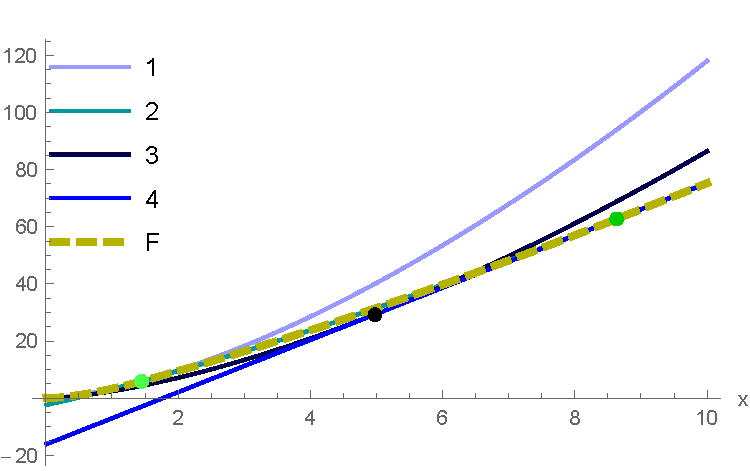
\includegraphics[width=\linewidth]{Prob3/eta007_1.pdf}
		\end{minipage}
		& \begin{minipage}{.4\textwidth}
			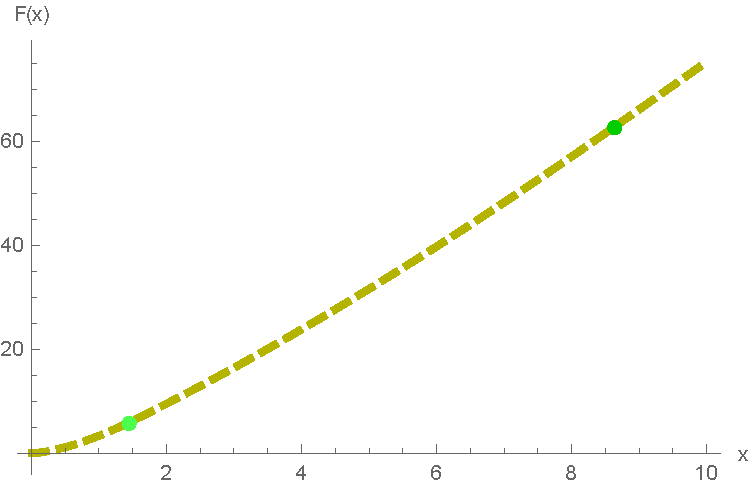
\includegraphics[width=\linewidth]{Prob3/eta007dash_1.pdf}
		\end{minipage}
		\\ \hline
		$\eta=0.012$ & 
		\begin{minipage}{.4\textwidth}
			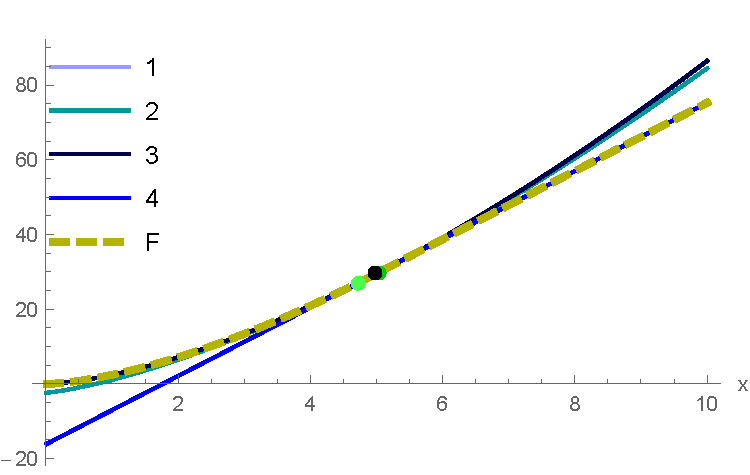
\includegraphics[width=\linewidth]{Prob3/eta0121_1.pdf}
		\end{minipage}
		& \begin{minipage}{.4\textwidth}
			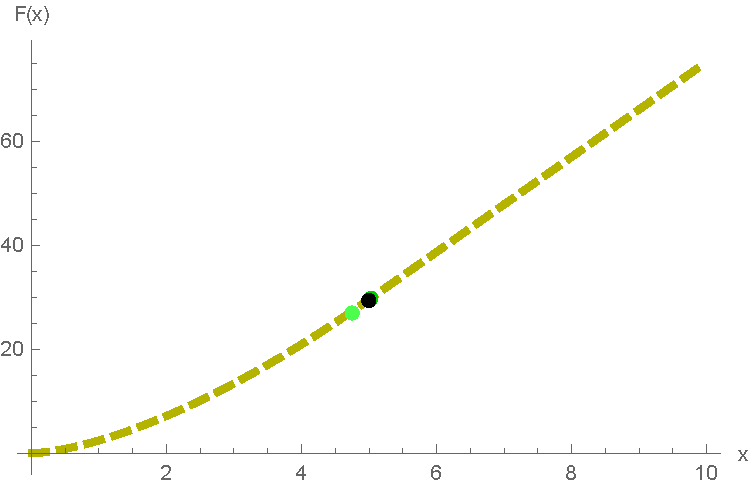
\includegraphics[width=\linewidth]{Prob3/eta012dash_1.pdf}
		\end{minipage}
		\\ \hline
		$\eta=0.013$ & \begin{minipage}{.4\textwidth}
			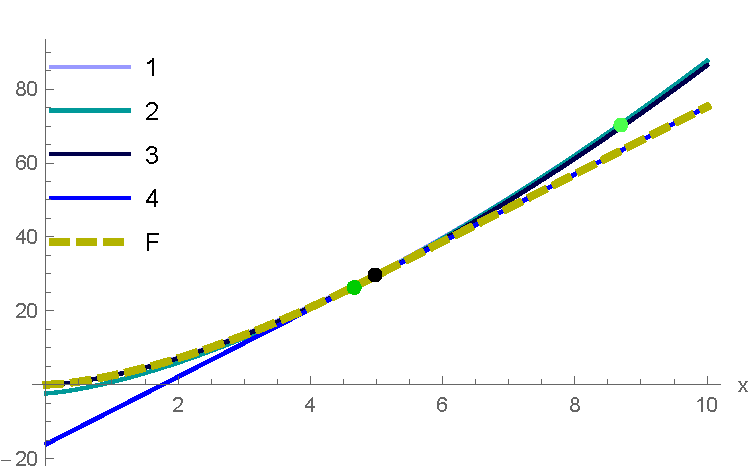
\includegraphics[width=\linewidth]{Prob3/eta013_1.pdf}
		\end{minipage}
		& \begin{minipage}{.4\textwidth}
			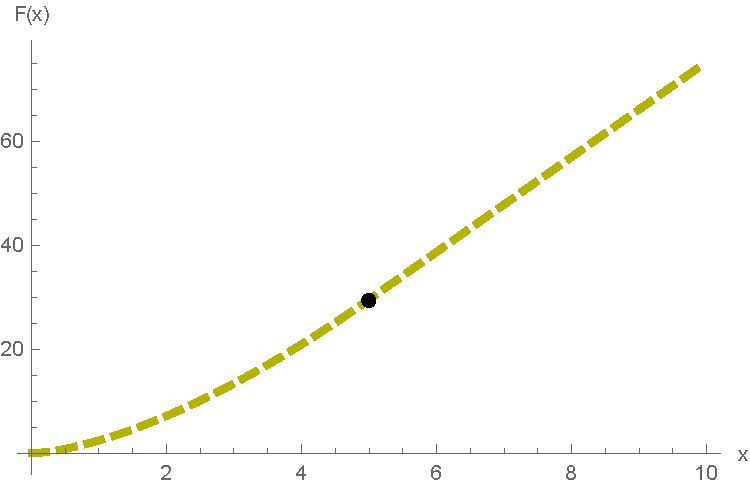
\includegraphics[width=\linewidth]{Prob3/eta013dash.pdf}
		\end{minipage} \\ \hline
	\end{tabular}
	\label{fig:3_F}
\end{table}

%\begin{figure}[!htb]
%	\begin{subfigmatrix}{6}
%		\subfigure[$\eta=0.007$ ]{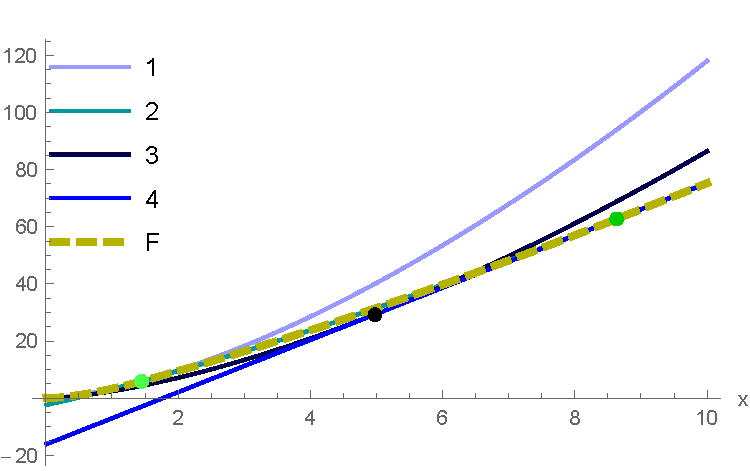
\includegraphics[width=0.32\textwidth]{Prob3/eta007_1.pdf}}
%		\subfigure[$\eta=0.012$ ]{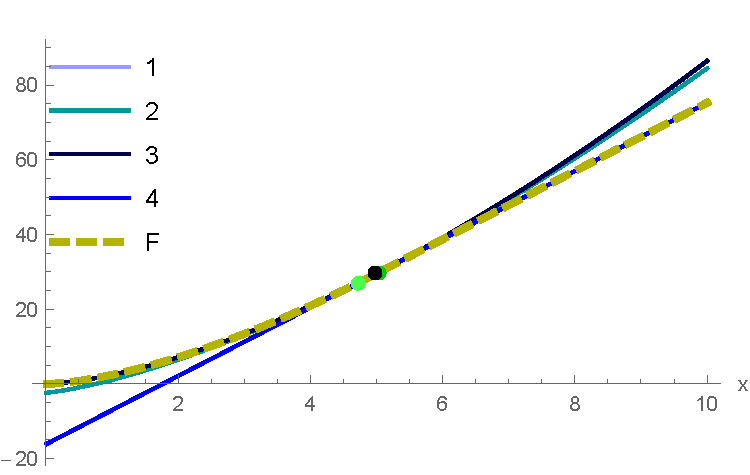
\includegraphics[width=0.32\textwidth]{Prob3/eta0121_1.pdf}}
%		\subfigure[$\eta=0.013$ ]{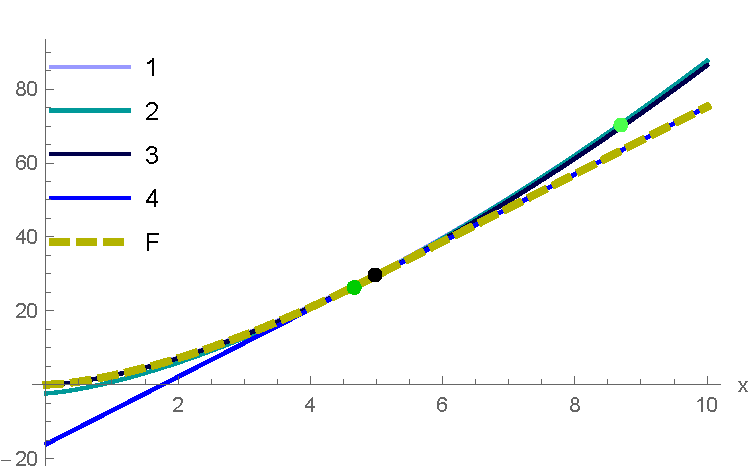
\includegraphics[width=0.32\textwidth]{Prob3/eta013_1.pdf}}
%		\subfigure[$\eta=0.007$]{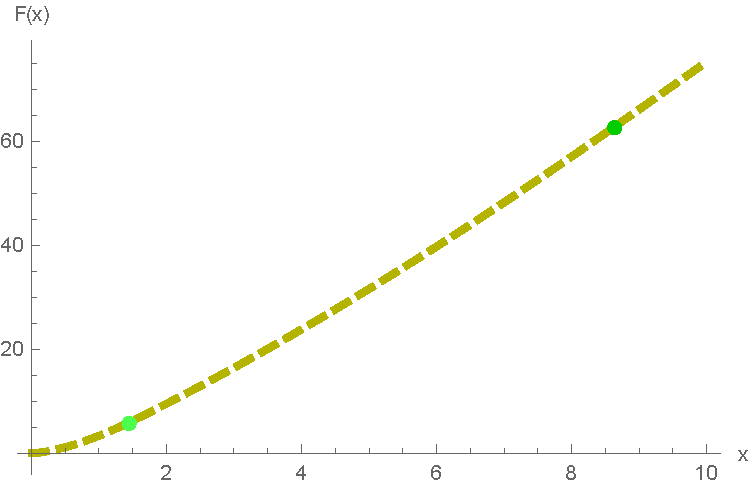
\includegraphics[width=0.32\textwidth]{Prob3/eta007dash_1.pdf}}
%		\subfigure[$\eta=0.012$]{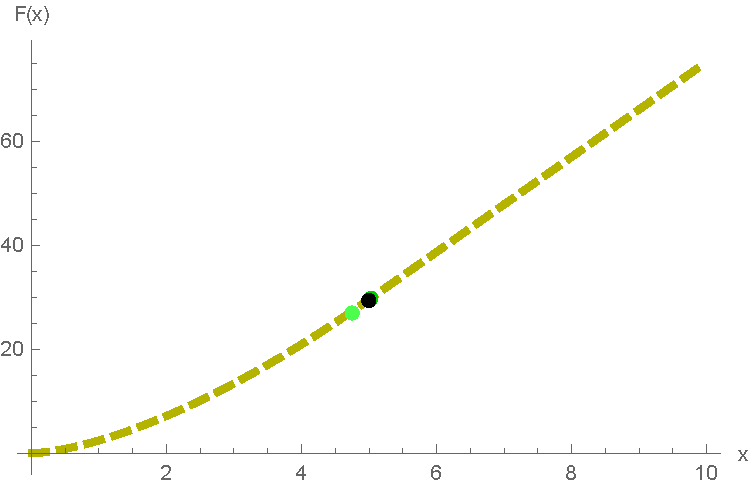
\includegraphics[width=0.32\textwidth]{Prob3/eta012dash_1.pdf}}
%		\subfigure[$\eta=0.013$]{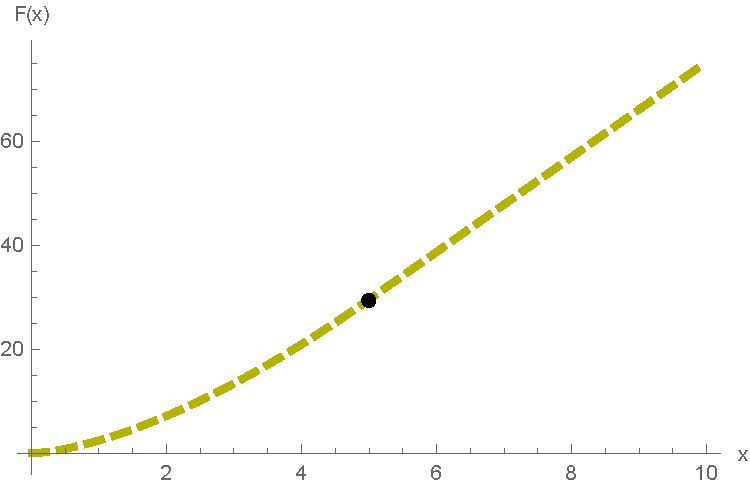
\includegraphics[width=0.32\textwidth]{Prob3/eta013dash.pdf}}
%	\end{subfigmatrix}
%	\caption{Value function $F$ minus $\frac{\pi_0}{r}$ and respective subfunctions, presented following the order in in \eqref{3_madzbigboy}, associated to different settings of parameter $\eta$. There is also represented the threshold values: $x^*_{1,A}$ (light green),  $x^*_2$ (darker green) and $x^*_{1,R}$ (black). }
%	\label{fig:3_F}
%\end{figure}

First, note that regarding this set of values, we obtain a cannibalisation threshold $\eta^*\simeq 0.0121$. 

Therefore in the situations represented on the first and second columns the firm is recommended to 
%we have, for the plots in the first and second columns, that it's better to 
invest and have a period of simultaneous production and to produce solely the \textit{new} product when the demand is observed to be $x^*_2$.
%only after the second threshold being reached, we change to produce solely the \textit{new} product.
On the other side, in the third column, it is represented the situation for which a firm should invest and replace immediately the \textit{old} established product by the \textit{new} one as soon as $x^*_{1,R}$ is hit.
%when we invest, we should immediately produce solely the \textit{new} product.

In the first row ($\eta=0.007$) we observe that the thresholds to be considered are $x_{1,A}^*$ and $x_2^*$. The first one states upon which demand level we should invest in the \textit{new} product and start the simultaneous production. The second one states upon which demand level we should produce only the \textit{new} product. The respective value function associated is defined by 3 parts, being given by 
\begin{equation}
\begin{split}
F(x)=\frac{\pi_0}{r}+
	a_{1,A}x^{d_1}  \mathds{1}_{ \{x<x^*_{1,A} \}}&+
	\left( a_2x^{d_1}+\frac{(\theta-\alpha K_1)K_1-2 \eta K_0 K_1}{r-\mu} x - \delta K_1 \right)  \mathds{1}_{ \{ x_{1,A} \leq x < x_2^* \}}\\
	&+
	\left(  \frac{(\theta-\alpha K_1)K_1 x}{r-\mu} -\frac{\pi_0}{r} - \delta K_1 \right)   \mathds{1}_{ \{ x>x_2^*  \} }.
\end{split}
	\label{3_F2t}
\end{equation}	

In the second row ($\eta=0.012$), we are in a similar situation as in the previous row, where we have two thresholds and the value function is also defined in three parts, as in \eqref{3_F2t}.
Observe also that as $\eta \to \eta^*$, the three thresholds tend to admit the same value. This is accordance with the analytical result that replacing $\eta$ by $\eta^*$ in $x^*_{1,A}$ \eqref{eq:3_x1A} and in $x^*_{1,R}$ \eqref{2_xB} we get
$$x^*_{1,A}(\eta^*)=x_2^*(\eta^*)=x^*_{1,R}.$$


In the third row, we observe that the threshold to be considered is $x_{1,R}^*$. In this case the value function is only defined by two parts, being given by
$$F(x)=\frac{\pi_0}{r}+
	a_{1,R}x^{d_1} \mathds{1}_{ \{ x<x_{1,R}^* \} }+
	\left(  \frac{(\theta-\alpha K_1)K_1 x}{r-\mu} -\frac{\pi_0}{r} - \delta K_1 \right)  \mathds{1}_{ \{ x>x_{1,R}^* \} }$$

\vspace{3mm}
On the next sections we analyse derived thresholds and how they are influenced by the parameters, first analytically and then numerically. 
Taking into account that the threshold regarding the immediate replace of the established product by the innovative when the investment is incurred ($x^*_{1,R}$) is the same as the one studied in the benchmark model of Chapter \ref{chapter:2}, we won't go further on it - analysis and conclusion were already stated on Section \ref{subsec:2_bm}.

The set of parameters now considered is the same as in previous chapters (more precisely Chapter \ref{chapter:2}). Additionally we choose $\eta=0.007$, guaranteeing that we are at the situation where $\eta <\eta^*$, that is, the firm relies on $x^*_{1,A}$ and $x^*_2$, since it's optimal to have a simultaneous production period.
\subsection{Demand threshold $x_{1,A}^*$}
\label{3_dmx1A}


\begin{prop}
	\label{3_propx1A}
	The decision threshold $x_{1,A}^*$ increases with $\eta, \ \delta, \ \sigma, \ \alpha, \ K_0$ and $K_1$ and decreases with $\theta$.
\end{prop}

\textbf{Proof:}

The results regarding parameters $\eta, \ \delta, \ \alpha $ and $\theta$ come immediately by the expression of $x_{1,A}^*$  \eqref{eq:3_x1A}.

Regarding $\sigma$, we obtain that
\begin{align*}
\frac{\partial x_{1,A}^* ( \sigma) }{\partial \sigma}=\frac{2 \delta  (\mu -r) \left(-2 \mu ^2+\mu  \sigma ^2 \left(\phi+1\right)-2 r \sigma ^2\right)}{(d_1-1)^2 \sigma ^5 \phi (\theta -\alpha  K_1 -2 \eta  K_0)}>0,
\end{align*}
From condition \eqref{3_cond} and the sign of the numerator in \eqref{1_xBs}, it follows, respectively, that the denominator and the numerator are positive.   %the denominator is positive since $d_1>1$, $\phi>0$ and the denominator is positive since $r>\mu$ and by noting that $-2 \mu ^2+\mu  \sigma ^2 \left(\phi+1\right)-2 r \sigma ^2<0 \Leftrightarrow \mu d_1-r<0$, which holds always, as previously showed in \eqref{mud1-r}.

Regarding $K_0$ and $K_1$, we obtain that
\begin{align*}
\frac{\partial x_{1,A}^* ( K_0) }{\partial K_0}&=\frac{2 \delta d_1 \eta  (r-\mu )}{(d_1-1) (-\theta +\alpha  K_1+2 \eta  K_0)^2}>0\\
\frac{\partial x_{1,A}^* ( K_1) }{\partial K_1}&=\frac{\alpha \delta d_1 \eta  (r-\mu )}{(d_1-1) (-\theta +\alpha  K_1+2 \eta  K_0)^2}>0,
\end{align*}
from which the result holds.
%Regarding parameters $\mu$ and $r$, we obtained complex derivates, from which we couldn't deduce any analytical result. However, as it will be showed hereunder, $x^*_C$ behaves in a non-monotonic way with all of them.
\begin{flushright}
	$\square$
\end{flushright}


We performed numerical experiments to assess the changes of $x^*_{1,A}$ with the different parameters. The results obtained are presented on Figures \ref{fig:2_x1Ai} and \ref{fig:2_x1Ad}.


\begin{figure}[!htb]
	\begin{subfigmatrix}{7}
		\subfigure[$\eta \in (0, \alpha )$ ]{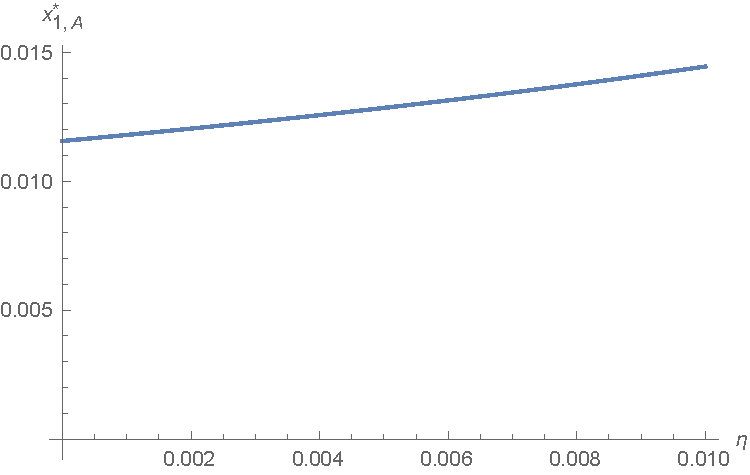
\includegraphics[width=0.32\textwidth]{Prob3/x1Aeta.pdf}}
		\subfigure[$\delta \in (1,2)$]{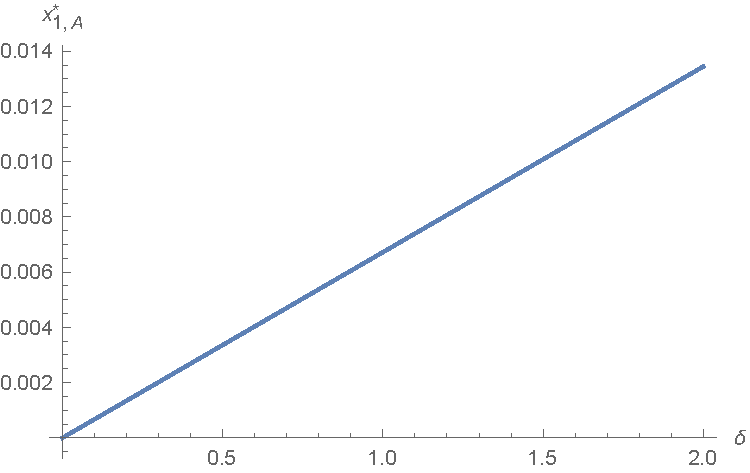
\includegraphics[width=0.32\textwidth]{Prob3/x1Adelta.pdf}}
		\subfigure[$\alpha \in (0, \min \{ 1/K_0, \theta/K_1 \} )$ ]{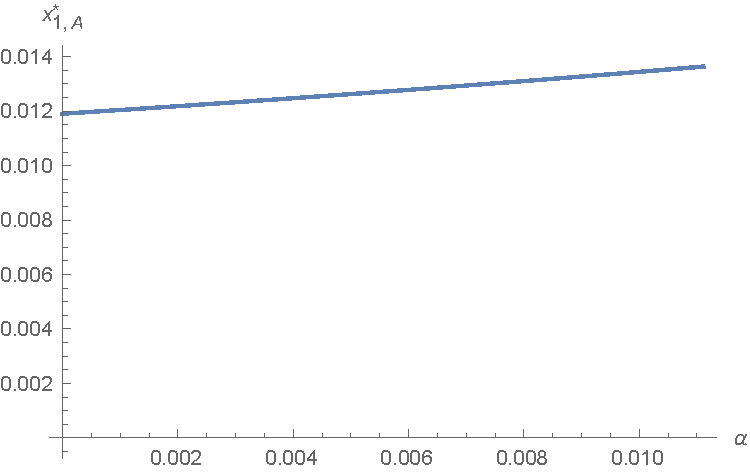
\includegraphics[width=0.32\textwidth]{Prob3/x1Aalpha.pdf}}
		\subfigure[$K_0 \in (0,1/\alpha)$]{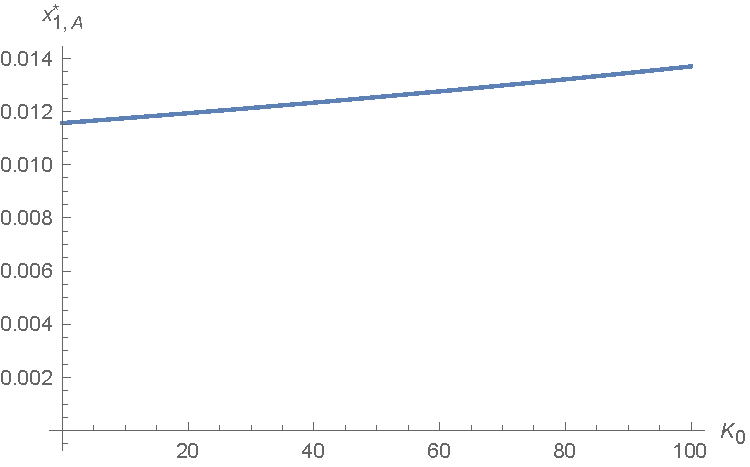
\includegraphics[width=0.32\textwidth]{Prob3/x1Ak0.pdf}}
		\subfigure[$K_1 \in (0,\theta/\alpha)$]{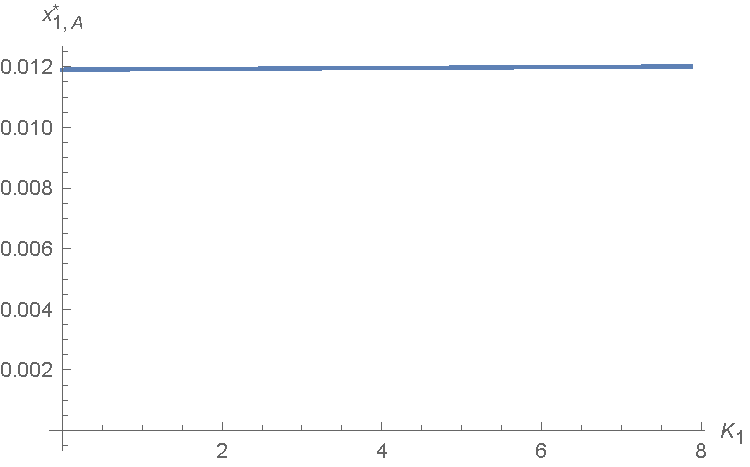
\includegraphics[width=0.32\textwidth]{Prob3/x1Ak1.pdf}}
		\subfigure[$\sigma \in (0,1)$]{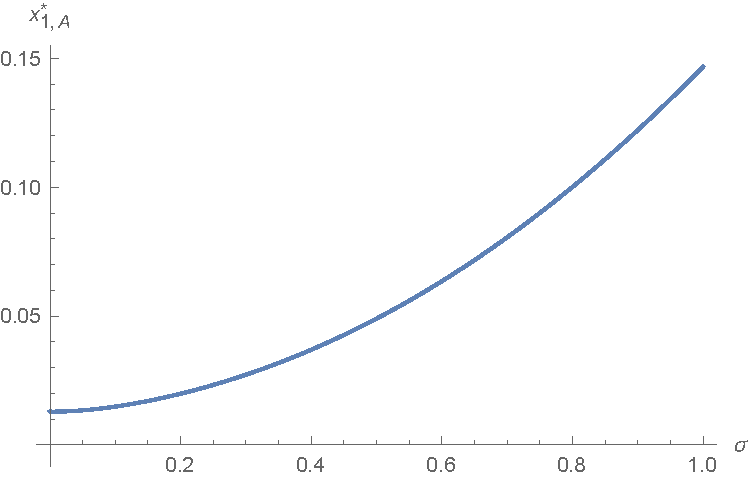
\includegraphics[width=0.32\textwidth]{Prob3/x1Asigma.pdf}}
		\subfigure[$r \in (0,\mu)$]{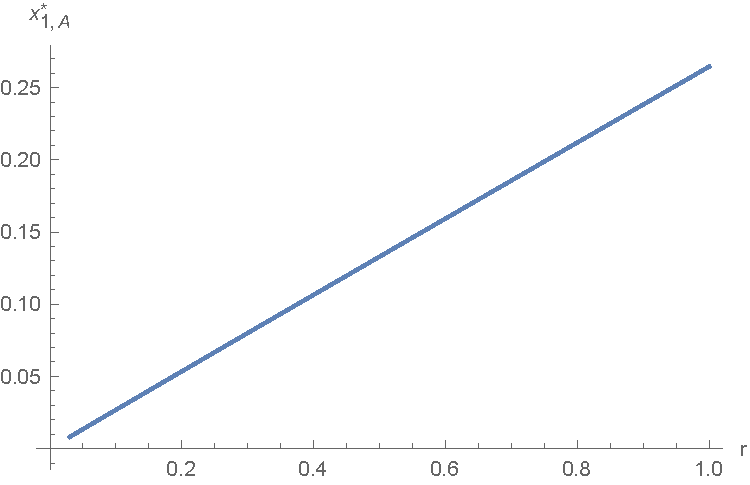
\includegraphics[width=0.32\textwidth]{Prob3/x1Ar.pdf}}
	\end{subfigmatrix}
	\caption{Behaviour of the threshold value $x^*_{1,A}$ with respect to the parameters with which it increases $\eta, \ \delta, \ \alpha, \ K_0, \ K_1, \ \sigma$ and $r$.}
	\label{fig:2_x1Ai}
\end{figure}

On Figure \ref{fig:2_x1Ai} (a) we observe that the larger the cannibalisation parameter, the later the firm is expected to adopt the new product, since a high demand needs to be observed such that the investment and associated costs of the simultaneous production are overcome. Recall that for quite large values of $\eta$, we are in the situation where is preferable to invest on the \textit{new} product, replacing immediately the \textit{old} one.

The linear relationship between $\delta$ and $x_{1,A}^*$, as presented on Figure \ref{fig:2_x1Ai} (b), comes immediately  by the threshold's expression. This is financially justified by the fact that a larger $\delta$ results on larger investmnet (sunk) costs and, therefore, the firm only invests when it could profit. 

One can note that $x^*_{1,A}$ shows a similar linear behaviour with $\alpha$, $K_0$ and $K_1$. 

On Figure \ref{fig:2_x1Ai} (c), the growth of $\alpha$ suggests that the established product is preferable to the \textit{new} one, resulting in a larger demand threshold.

Concerning both capacities of production $K_0$ and $K_1$, we observe on Figures \ref{fig:2_x1Ai} (d) and (e), that the larger they are, the higher the demand level that triggers the invest is. Regarding $K_0$ this result is justified by the fact that the larger is the value it takes, the higher the profit of the established product is, so the firm gets more relutant about investing for low demand levels. In different circumstances, a larger $K_1$ induces a longer investment (so as investment costs), wherefore the investment decision will only incur if the observed demand is large enough. 



Once again we observe on Figure \ref{fig:2_x1Ai} (f) that a growth uncertainty on the demand lead to the postponement of the investment decision. 

Although we weren't able to deduce any analytical result concerning the interest rate, we obtain on Figure \ref{fig:2_x1Ai} (g) that, as already stated, an increasing interest rate delays the investment decision.

%On Figure \ref{fig:2_x1Ai} we present numerical  comprove what was stated on Proposition \ref{3_propx1A}. We also add another one, regarding the discount rate $r$, for which we couldn't derive any analytical solution, but studying the behaviour of $x^*_{1,A}$ we conclude that it also increases with $r$.

\begin{figure}[!htb]
	\begin{subfigmatrix}{2}
		\subfigure[$\mu \in (0,r)$]{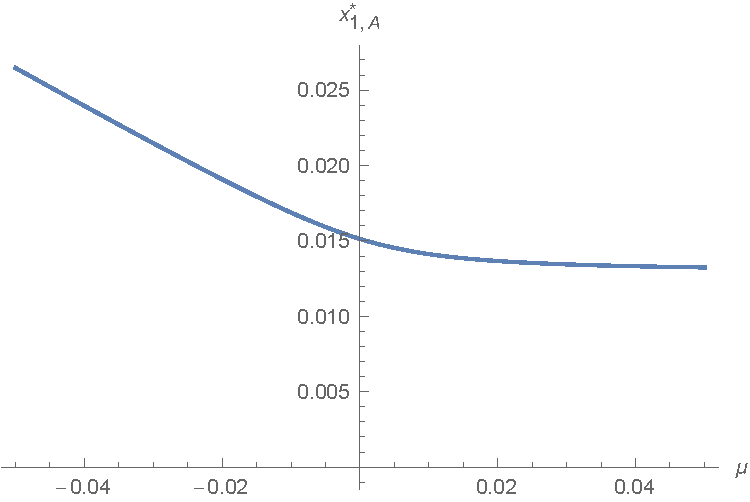
\includegraphics[width=0.4\textwidth]{Prob3/x1Amu.pdf}}
		\subfigure[$\theta \in (1,10)$]{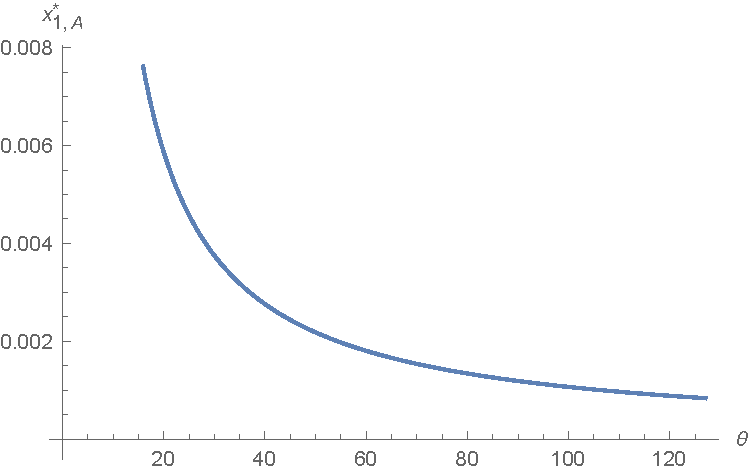
\includegraphics[width=0.4\textwidth]{Prob3/x1Atheta.pdf}}
	\end{subfigmatrix}
	\caption{Behaviour of the threshold value $x^*_{1,A}$ with respect to parameters with which it decreases $\mu$ and $\theta$.}
	\label{fig:2_x1Ad}
\end{figure}


As analysed on previous chapters, we observe on a declining market ($\mu<0$), the investment threshold decreases linearly in a stronger rate than in a growing market $\mu>0$, on which the threshold barely changes.
 
Finally, in view of Figure \ref{fig:2_x1Ai}, we obtain that the larger the innovation level, the higher is the expected profit during the simultaneous production period and, hence, the more attractive is the investment on the \textit{new} product.
%On Figure \ref{fig:2_x1Ad} we present some plots that also comprove what was stated on Proposition \ref{3_propx1A}, but with respect to the parameters with which $x_{1,A}^*$ increases. Again, we add the plot concerning the drift parameter $\mu$, for which we couldn't derive any analytical solution, but studying the behaviour of $x^*_{1,A}$ we conclude that it also decreases with $\mu$.


%\subsection{Demand threshold $x_{1,R}^*$}
%\label{3_dmx1R}

%All results come from Section \ref{2_bm} and thus they won't repeated here.



\subsection{Demand threshold $x_2^*$}
	\label{3_dmx2}
	
\begin{prop}
	\label{3_propx2}
	The decision threshold $x_2^*$ increases with $\sigma$ and decreases with $\eta, \ \alpha, \ K_0$ and $K_1$.
\end{prop}

\textbf{Proof:}

The results regarding parameters $\eta, \ \alpha, \ K_0$ and $K_1$ come immediately by the expression of $x_2^*$  \eqref{3:x2}.

Regarding $\sigma$, we obtain that
\begin{align*}
\frac{\partial x_2^* ( \sigma) }{\partial \sigma}=
\frac{(\alpha  K_0-1) (r-\mu) \left(-2 \mu ^2+\mu  \sigma ^2 \left(\phi+1\right)-2 r \sigma ^2\right)}{(d_1-1)^2 \eta  K_1 r \sigma ^5 \phi}>0
\end{align*}
since the denominator is positive and the numerator also, concerning the same reason used in \eqref{1_xBs}.
%where the denominator is positive since $d_1>1$, $\phi>0$  and the denominator is positive since $r>\mu$, $1-\alpha K_0>0$ and by noticing (again) that $-2 \mu ^2+\mu  \sigma ^2 \left(\phi+1\right)-2 r \sigma ^2<0 \Leftrightarrow \mu d_1-r<0$, which holds always, as previously showed in \eqref{mud1-r}.

%Regarding parameters $\mu$ and $r$, we obtained complex derivates, from which we couldn't deduce any analytical result. However, as it will be showed hereunder, $x^*_C$ behaves in a non-monotonic way with all of them.
\begin{flushright}
	$\square$
\end{flushright}


Unfortunately we are not able to derive any analytical expression regarding changes influenced by the discount rate and demand's drift. However, supporting on numerical experiments we observe that the behaviour hereunder described holds.
%Considering the same parameters as in Section \ref{3_dmx1A}, we perform some numerical approximations concerning $x_2^*$.

\begin{figure}[!htb]
	\begin{subfigmatrix}{1}
		\subfigure[$\sigma \in (0, 1 )$ ]{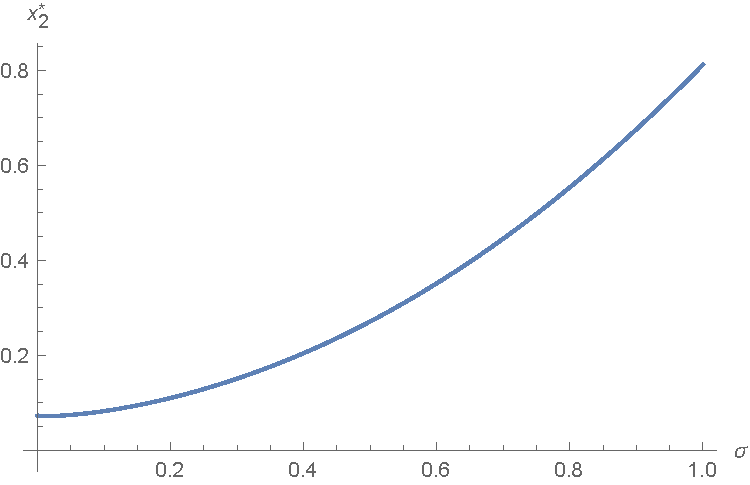
\includegraphics[width=0.45\textwidth]{Prob3/x2sigma.pdf}}
	\end{subfigmatrix}
	\caption{Behaviour of the threshold value $x^*_2$ with respect to the parameter with which it increases $\sigma$.}
	\label{fig:2_x2i}
\end{figure}

%From Figure \ref{fig:2_x2i} we comprove what was stated on Proposition \ref{3_propx2} regarding $\sigma$. 

%We also obtained that the volatility $\sigma$ was the unique parameter we found to increase both thresholds $x_{1,A}^*$ and $x_2$. Note that by Section \ref{2_bm}, that the same holds for the threshold $x_{1,R}$. Thus we conclude that a situation where the demands shows to have a high volatility, both investment and replacement decisions tend to be postponed.

Interestingly, market's uncertainty is the unique aspect that delays the abandonment of the production of the \textit{old} product, being preferable to keep the firm producing both products. This result is presented on Figure \ref{fig:2_x2i} and it is justified by the fact that the stable profit associated to the \textit{old} product, which is not influenced by the uncertainty of the market, benefits the firm from possible low demand levels, leading to a low profit, if the firm was only producing the innovative product.

\begin{figure}[!htb]
	\begin{subfigmatrix}{6}
		\subfigure[$\eta \in (0, \alpha )$ ]{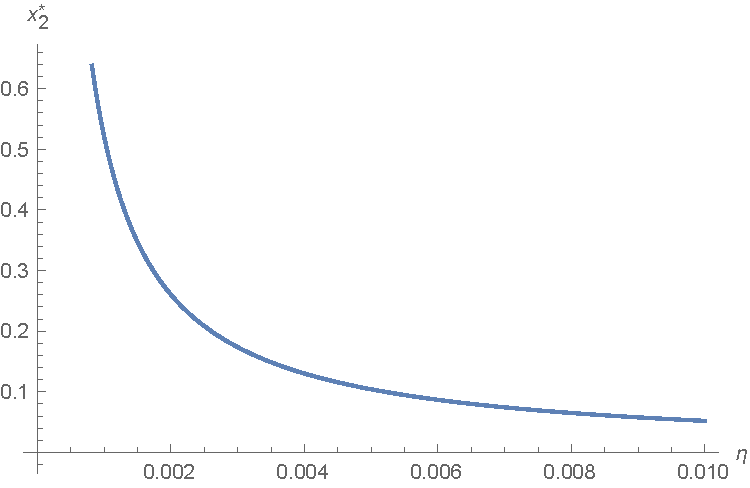
\includegraphics[width=0.32\textwidth]{Prob3/x2eta.pdf}}
		\subfigure[$\alpha \in (0, \min \{ 1/K_0, \theta/K_1 \} )$ ]{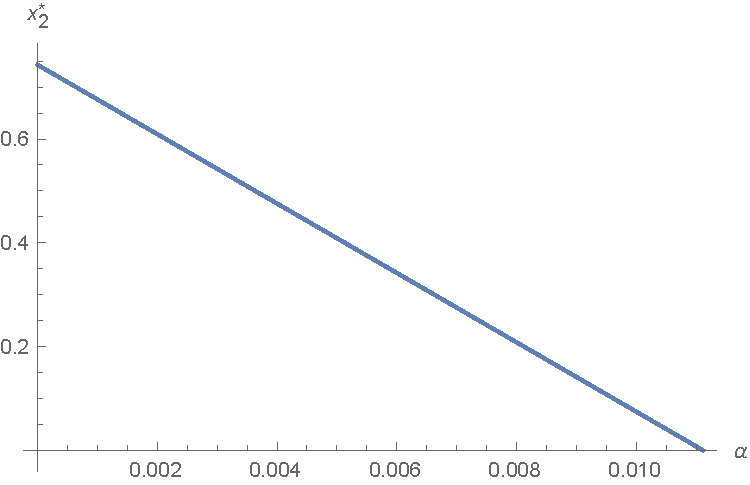
\includegraphics[width=0.32\textwidth]{Prob3/x2alpha.pdf}}
		\subfigure[$K_0 \in (0,1/\alpha)$]{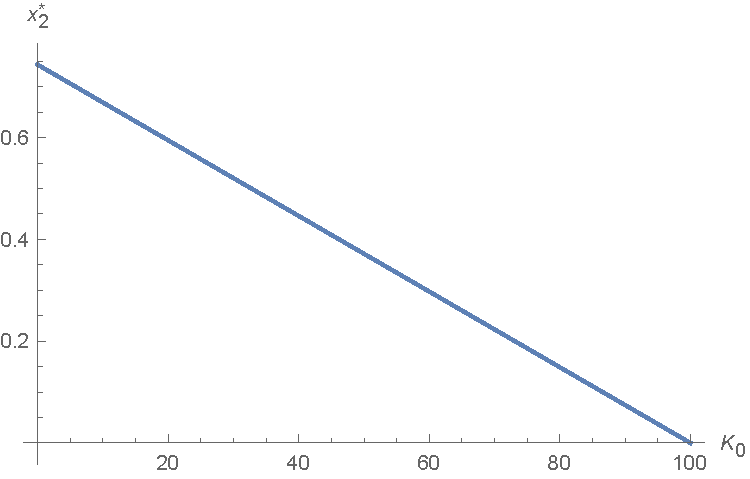
\includegraphics[width=0.32\textwidth]{Prob3/x2k0.pdf}}
		\subfigure[$K_1 \in (0,\theta/\alpha)$]{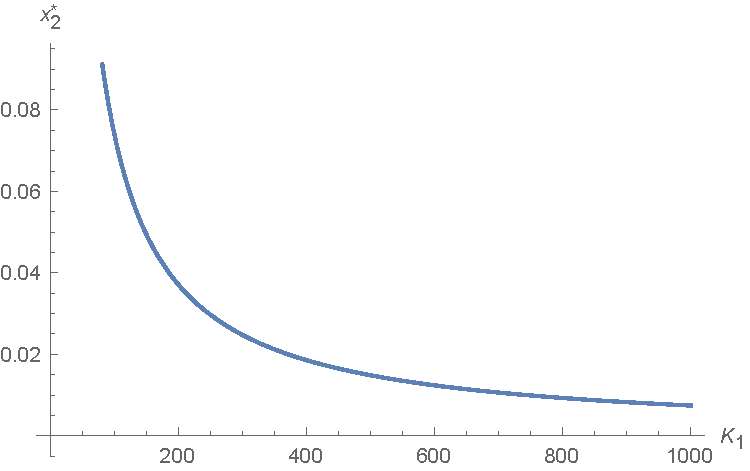
\includegraphics[width=0.32\textwidth]{Prob3/x2k.pdf}}
		\subfigure[$r \in (0,\mu)$]{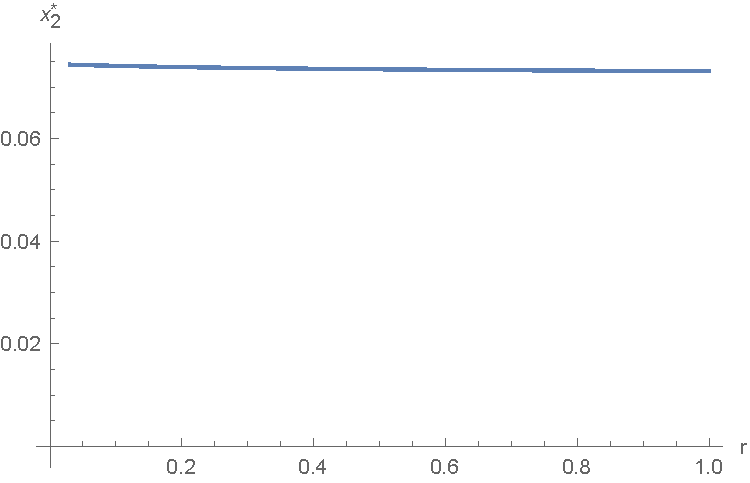
\includegraphics[width=0.32\textwidth]{Prob3/x2r.pdf}}
		\subfigure[$\mu \in (0,r)$]{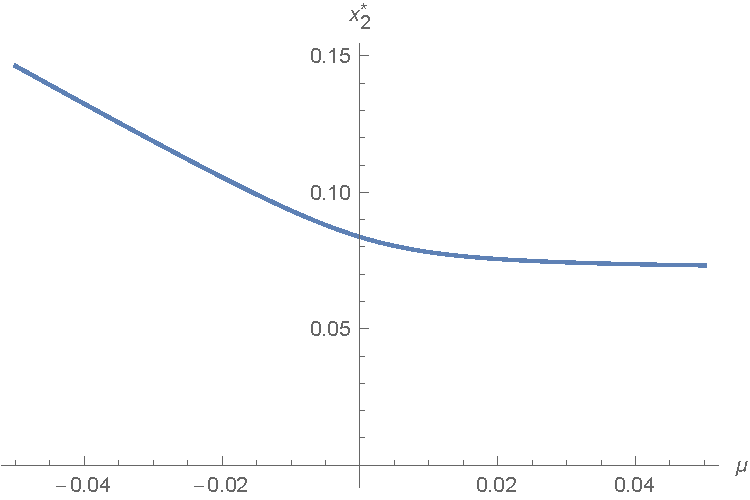
\includegraphics[width=0.32\textwidth]{Prob3/x2mu.pdf}}
	\end{subfigmatrix}
	\caption{Behaviour of the threshold value $x^*_{1,A}$ with respect to parameters with which it decreases $\eta, \ \alpha, \ K_0, \ K_1, \ r$ and $\mu$.}
	\label{fig:2_x2d}
\end{figure}

In view of Figure \ref{fig:2_x2d} (a) the larger the cannibalisation parameter considered, the smaller is the profit obtained during the simultaneous production period, inducing the firm to antecipate the abandonment decision. 

Since both cannibalisation $\eta$ and capacity $K_1$ appear in the denominator of $x^*_2$, a similar behaviour is expected from both them. This is verified on Figure \ref{fig:2_x2d} (d) and comes from the fact that a larger capacity investment (already) incurred - when the demand reached $x^*_{1,A}$ - results on smaller profit by considering a simultaneous production than by solely producing the innovative product, encouraging the firm to invest earlier.

By confronting the results presented on Figures \ref{fig:2_x2d} (b) and (c) with the expression on \eqref{3:x2}, we observe that both $\alpha$ and $K_0$ have an akin linear effect: the larger the sensibility $\alpha$ or the capacity $K_0$, the earlier the firm should cease the production of the \textit{old} product.

Once again we obtain the same peculiar type of behaviour with respect to changes on market's fortuity, as is showed on Figure \ref{fig:2_x2d} (f).




%On Figure \ref{fig:2_x2d} we show how the threshold $x_2$ decreases with parameters stated on Proposition \ref{3_propx2}. We also add plots concerning the drift parameter $\mu$ and the discount rate $r$, for which we couldn't derive any analytical solution, but studying how $x^*_2$ behaves with them, we conclude that it also increases with $\mu$ and $r$, from which the behaviour showed may be generalized.
